\documentclass[tikz,border=0pt]{standalone}
\usepackage{tikz}
\usepackage{amsmath}

% Colors matching blog _variables.scss
\definecolor{bg}{HTML}{1E1E1E}
\definecolor{textlight}{HTML}{ECECEC}
\definecolor{circlelight}{HTML}{D4D4D4}
\definecolor{muted}{HTML}{858585}
\definecolor{errbar}{HTML}{B4B4B4}
\definecolor{shblue}{HTML}{569CD6}
\definecolor{omegablue}{HTML}{8ABBE6}
\definecolor{shcoral}{HTML}{E06C60}

\begin{document}
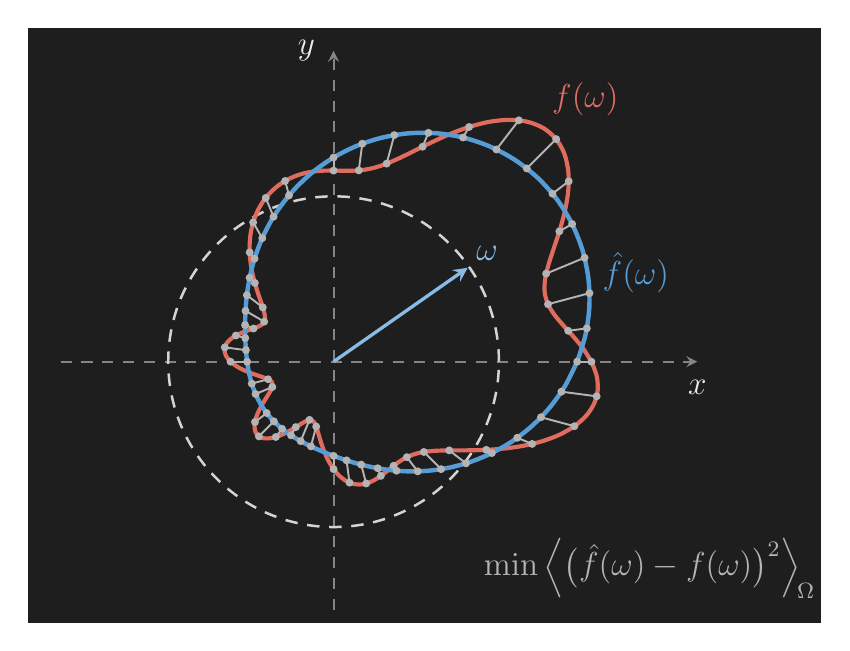
\begin{tikzpicture}[
    scale=2.1,
    >=stealth,
    font=\large
]
    % Tighter bounding box around the diagram so it renders larger on the page
    \path[use as bounding box] (-1.85,-1.58) rectangle (2.95,2.02);
    \fill[bg] (-1.85,-1.58) rectangle (2.95,2.02);

    % Coordinate axes (dashed)
    \draw[->, dashed, color=muted, line width=0.75pt, dash pattern=on 4pt off 3.5pt]
        (-1.65,0) -- (2.20,0)
        node[below, color=textlight, yshift=-3pt] {$x$};
    \draw[->, dashed, color=muted, line width=0.75pt, dash pattern=on 4pt off 3.5pt]
        (0,-1.50) -- (0,1.88)
        node[left, color=textlight, xshift=-3pt] {$y$};

    % Unit circle (dashed, r = 1 removed)
    \draw[dashed, color=circlelight, line width=0.9pt, dash pattern=on 4.5pt off 3.5pt]
        (0,0) circle (1.0);

    % Unit direction vector \omega (shortened to touch the unit circle, label at tip)
    \draw[->, color=omegablue, line width=1.2pt] (0,0) -- (35:0.99);
    \node[color=omegablue, anchor=south west, inner sep=1.5pt] at (35:1.02) {$\omega$};

    % True directional function f(\omega) (drawn BEFORE error bars so error bars sit on top)
    \draw[color=shcoral, line width=1.5pt, line join=round]
        plot[domain=0:360, samples=121, smooth, variable=\t]
        (\t : {0.95 + 0.58*cos(\t - 35) + 0.14*cos(2*(\t - 35)) + 0.15*cos(6*(\t - 48)) + 0.08*sin(5*(\t - 35)) - 0.05*cos(8*(\t - 20))}) -- cycle;

    % Smooth polynomial approximation \hat{f}(\omega) (drawn BEFORE error bars so error bars sit on top)
    \draw[color=shblue, line width=1.6pt, line join=round]
        plot[domain=0:360, samples=61, smooth, variable=\t]
        (\t : {0.95 + 0.58*cos(\t - 35) + 0.14*cos(2*(\t - 35))}) -- cycle;

    % Radial least-squares residual bars & endpoint dots drawn ON TOP of the function curves
    % Spaced every 7.5 degrees (48 radial error bars around the circle)
    \foreach \t in {0, 7.5, ..., 352.5} {
        \pgfmathsetmacro{\rfhat}{0.95 + 0.58*cos(\t - 35) + 0.14*cos(2*(\t - 35))}
        \pgfmathsetmacro{\rf}{\rfhat + 0.15*cos(6*(\t - 48)) + 0.08*sin(5*(\t - 35)) - 0.05*cos(8*(\t - 20))}
        \pgfmathsetmacro{\diff}{abs(\rf - \rfhat)}
        \ifdim \diff pt > 0.03pt
            \draw[color=errbar, line width=0.7pt] (\t:\rfhat) -- (\t:\rf);
            \fill[color=errbar] (\t:\rf) circle (0.024);
            \fill[color=errbar] (\t:\rfhat) circle (0.024);
        \fi
    }

    % Direct curve labels (no arrows, placed cleanly beside each curve)
    % At \t = 48.5 deg: coral curve crest is at r_f = 1.896
    \node[color=shcoral, anchor=south west, inner sep=2pt] at (48.5:1.94) {$f(\omega)$};

    % At \t = 18.75 deg: blue curve is on the outside at \hat{r} = 1.625 (while coral curve dips inside to 1.39)
    \node[color=shblue, anchor=west, inner sep=2pt] at (18.75:1.68) {$\hat{f}(\omega)$};

    % Compact optimization objective in the bottom right, colored to match the residual/error bars (no arrow)
    \node[color=errbar, anchor=west] (objlabel) at (0.85, -1.25)
        {$\min \left\langle \big(\hat{f}(\omega) - f(\omega)\big)^2 \right\rangle_{\!\Omega}$};

\end{tikzpicture}
\end{document}
